\subsubsection{Overview}
\label{Alpha Synapse}
\index{Alpha Synapse}\index{utilities, Alpha Synapse}
\begin{figure}[h]
\begin{center}
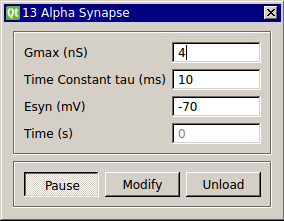
\includegraphics[width=2in]{alphasynapse.png} 
\caption[Alpha Synapse]{Creates an artificial synapse described by an alpha function.} 
\end{center}
\label{alphasynapse}
\end{figure}

This module creates an artificial synapse where the fixed conductance change is described by an alpha function. The fixed conductance waveform is pre-computed according to: \begin{equation}G = Gmax*\frac{t}{\tau}*exp[\frac{-(t-\tau)}{\tau}]\end{equation}
The current is computed according to Ohm's Law: \begin{equation}I_{syn} = G*(V_m-E_{syn})\end{equation}
This conductance is triggered by an event indicated by a value of "1" on input(1).

\subsubsection{Input Channels}
\begin{description}
\item[input(0)- Vm] membrane potential
\item[input(1) - Spike State] spike state (=1 to trigger synapse)
\end{description}

\subsubsection{Output Channels}
\begin{description}
\item[output(0) - ISyn] output current (A)
\end{description}

\subsubsection{Parameters}
\begin{description}
\item[Gmax] max. synaptic conductance for stimulus (nS)
\item[tau] time constant for alpha-shaped conductance (ms)
\item[Esyn] reversal potential for conductance (mV)
\end{description}